%\VignetteKeywords{genomation}
%\VignettePackage{genomation}
%\VignetteEngine{knitr::knitr}
%\VignetteIndexEntry{genomation: User Guide}
% !Rnw weave = knitr
\documentclass{article}\usepackage[]{graphicx}\usepackage[]{color}
%% maxwidth is the original width if it is less than linewidth
%% otherwise use linewidth (to make sure the graphics do not exceed the margin)
\makeatletter
\def\maxwidth{ %
  \ifdim\Gin@nat@width>\linewidth
    \linewidth
  \else
    \Gin@nat@width
  \fi
}
\makeatother

\definecolor{fgcolor}{rgb}{0.345, 0.345, 0.345}
\newcommand{\hlnum}[1]{\textcolor[rgb]{0.686,0.059,0.569}{#1}}%
\newcommand{\hlstr}[1]{\textcolor[rgb]{0.192,0.494,0.8}{#1}}%
\newcommand{\hlcom}[1]{\textcolor[rgb]{0.678,0.584,0.686}{\textit{#1}}}%
\newcommand{\hlopt}[1]{\textcolor[rgb]{0,0,0}{#1}}%
\newcommand{\hlstd}[1]{\textcolor[rgb]{0.345,0.345,0.345}{#1}}%
\newcommand{\hlkwa}[1]{\textcolor[rgb]{0.161,0.373,0.58}{\textbf{#1}}}%
\newcommand{\hlkwb}[1]{\textcolor[rgb]{0.69,0.353,0.396}{#1}}%
\newcommand{\hlkwc}[1]{\textcolor[rgb]{0.333,0.667,0.333}{#1}}%
\newcommand{\hlkwd}[1]{\textcolor[rgb]{0.737,0.353,0.396}{\textbf{#1}}}%

\usepackage{framed}
\makeatletter
\newenvironment{kframe}{%
 \def\at@end@of@kframe{}%
 \ifinner\ifhmode%
  \def\at@end@of@kframe{\end{minipage}}%
  \begin{minipage}{\columnwidth}%
 \fi\fi%
 \def\FrameCommand##1{\hskip\@totalleftmargin \hskip-\fboxsep
 \colorbox{shadecolor}{##1}\hskip-\fboxsep
     % There is no \\@totalrightmargin, so:
     \hskip-\linewidth \hskip-\@totalleftmargin \hskip\columnwidth}%
 \MakeFramed {\advance\hsize-\width
   \@totalleftmargin\z@ \linewidth\hsize
   \@setminipage}}%
 {\par\unskip\endMakeFramed%
 \at@end@of@kframe}
\makeatother

\definecolor{shadecolor}{rgb}{.97, .97, .97}
\definecolor{messagecolor}{rgb}{0, 0, 0}
\definecolor{warningcolor}{rgb}{1, 0, 1}
\definecolor{errorcolor}{rgb}{1, 0, 0}
\newenvironment{knitrout}{}{} % an empty environment to be redefined in TeX

\usepackage{alltt}
\usepackage{geometry}
\usepackage{wrapfig}

\geometry{verbose,tmargin=2.5cm,bmargin=2.5cm,lmargin=2.5cm,rmargin=2.5cm}


\title{genomation - a toolkit for annotation and visualization of genomic data}

\author{Altuna Akalin\\ \texttt{altuna.akalin@fmi.ch}\\
\and
Vedran Franke \\ \texttt{vedran.franke@gmail.com} }




\newcommand{\Rpackage}[1]{{\textit{#1}}}





\IfFileExists{upquote.sty}{\usepackage{upquote}}{}

\begin{document}
\maketitle
\tableofcontents

% ----------------------------------------------------------------- %
\section{Introduction}

Recent advances in sequencing technologies have enabled a downpoor of biological data. The sheer amount of data has impeeded the extraction of useful knowledge and novel hypothesis generation.
\begin{wrapfigure}{r}{0.4\textwidth}
 \vspace{-20pt}
  \begin{center}
    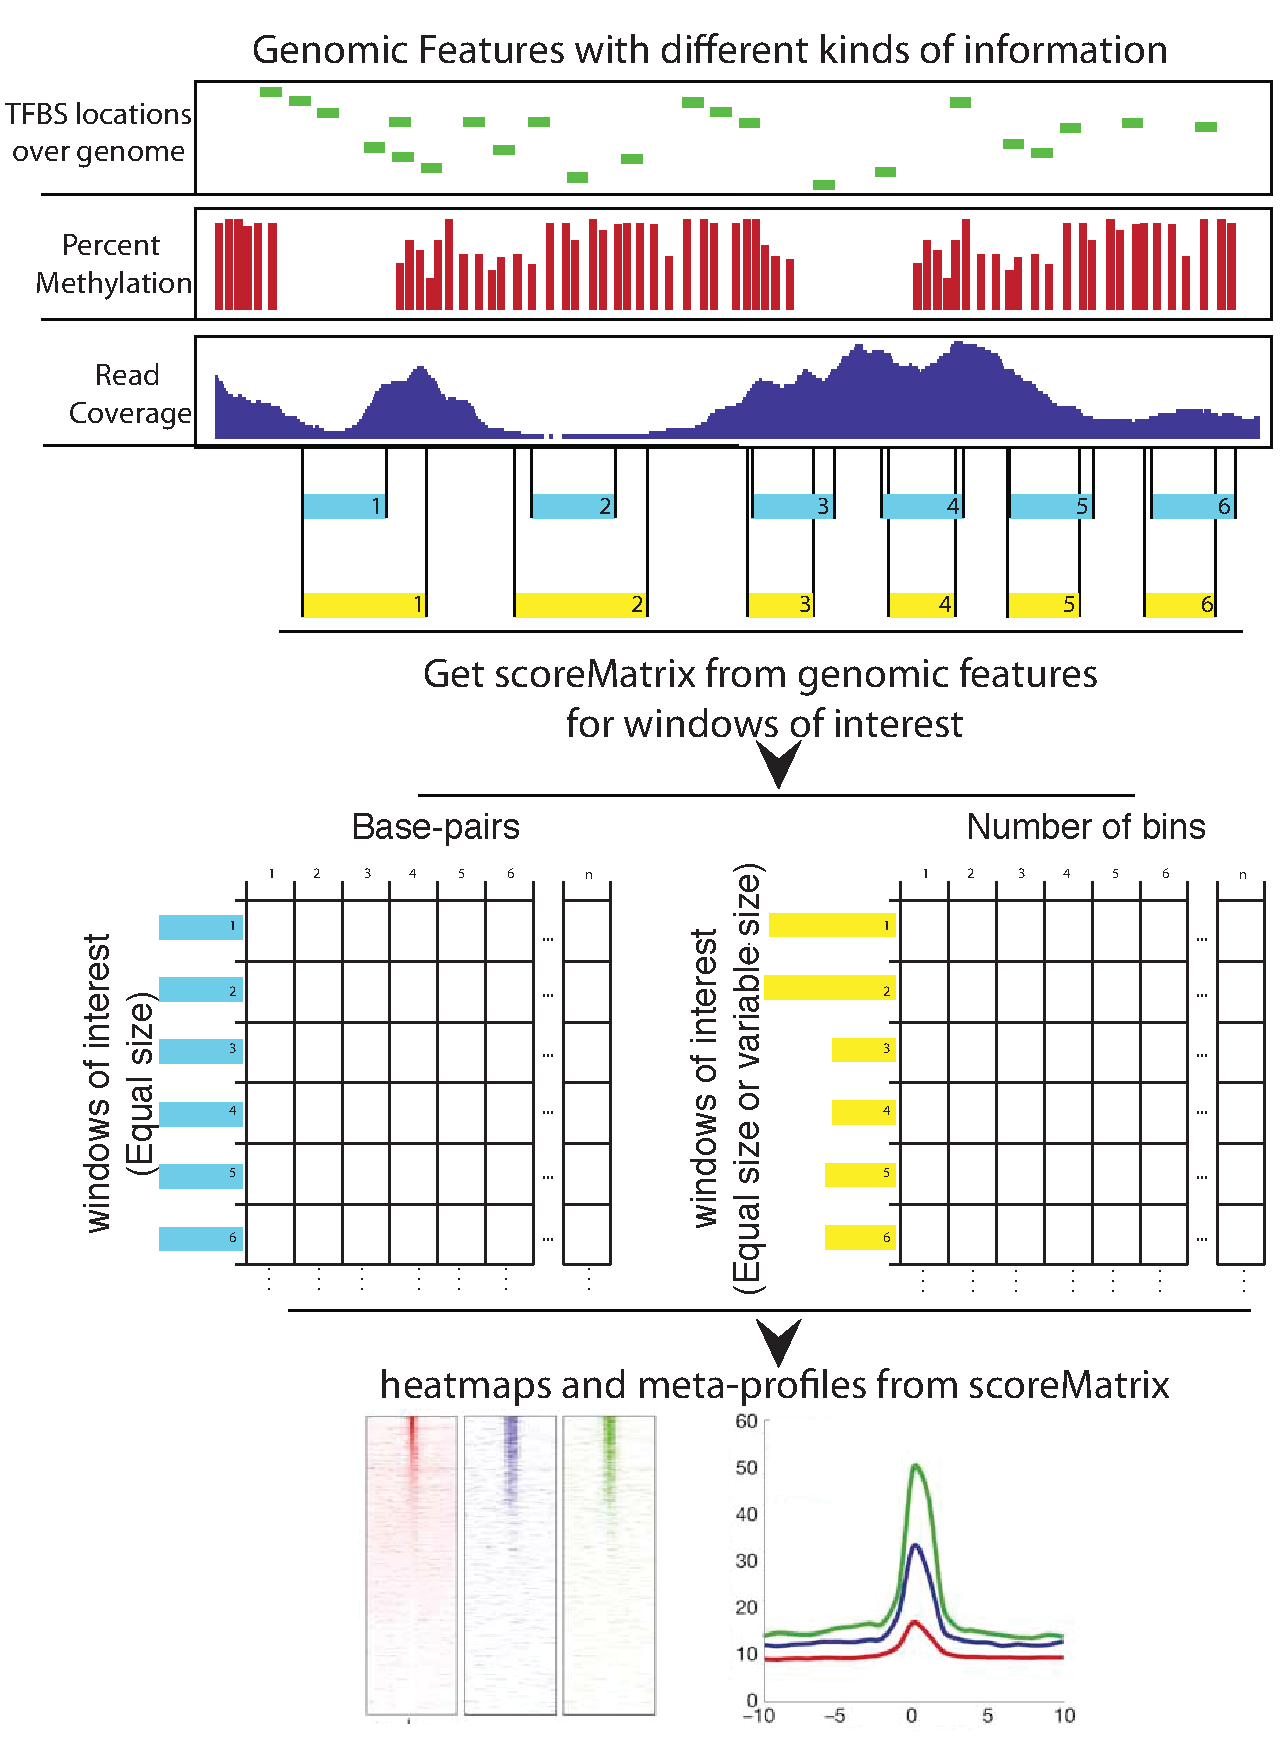
\includegraphics[width=0.4\textwidth]{Figures/genomationFlowChart1.pdf}
  \end{center}
  \caption{Bulk visualization for different genomic feature datasets flowchart}
   \vspace{-20pt}
\end{wrapfigure} 
\Rpackage{genomation} is a toolkit for annotation and in bulk visualization of 
genomic features (scored or unscored) over predefined regions. The \textbf{genomic features} the package can handle can be  anything with a minimal information of chromosome,start and end. The features could have any length
and most of the time they are associated with a score. Typical examples of such data sets include aligned reads from high-throughput sequencing (HTS) experiments, percent
methylation values for CpGs (or other cytosines), locations of transcription factor binding site motifs, and so on. On the other hand, throughout the vignette we use the phrase "genomic annotation" to refer to the regions of the genome associated with a potential function and do not necessarily have a score (examples: CpG islands, genes, enhancers, promoter, exons, etc. ). These genomic annotations are usually the regions of interest, and distribution of genomic features over/around the annotations are can make the way for biological interpretation of the data.


The pipeline for computational knowledge extraction consists of three steps: data filtering, integration of data from multiple sources or generation of predictive models and biological interpretation of produced models, which leads to novel hypotheses that can be tested in the wetlab. \Rpackage{genomation} aims to facilitate the integration of multiple sources of genomic features with genomic annotation or already published experimental results.
\\*

% ----------------------------------------------------------------- %
\section{Access the data}

High-throughput data which will be used to show the functonality of the \Rpackage{genomation} is located in two places. The annotation and cap analysis of gene expression (CAGE) data comes prepared with the genomation package, while the raw HTS data can be found in the sister package \Rpackage{genomationData}.\\
To install the \Rpackage{genomation} and the complementary data package the from the github repository c/p the following lines into your R interpreter:
\begin{knitrout}
\definecolor{shadecolor}{rgb}{0.969, 0.969, 0.969}\color{fgcolor}\begin{kframe}
\begin{alltt}
\hlkwd{library}\hlstd{(devtools)}
\hlkwd{install_github}\hlstd{(}\hlstr{"genomationData"}\hlstd{,} \hlkwc{username} \hlstd{=} \hlstr{"frenkiboy"}\hlstd{)}
\hlkwd{install_github}\hlstd{(}\hlstr{"genomation"}\hlstd{,} \hlkwc{username} \hlstd{=} \hlstr{"frenkiboy"}\hlstd{)}
\end{alltt}
\end{kframe}
\end{knitrout}


The \Rpackage{genomationData} vignette contains a verbose description of contained files.\\
To list the available data:
\begin{knitrout}
\definecolor{shadecolor}{rgb}{0.969, 0.969, 0.969}\color{fgcolor}\begin{kframe}
\begin{alltt}
\hlkwd{list.files}\hlstd{(}\hlkwd{system.file}\hlstd{(}\hlstr{"extdata"}\hlstd{,} \hlkwc{package} \hlstd{=} \hlstr{"genomationData"}\hlstd{))}
\end{alltt}
\end{kframe}
\end{knitrout}


To see the descriptions of the files:
\begin{knitrout}
\definecolor{shadecolor}{rgb}{0.969, 0.969, 0.969}\color{fgcolor}\begin{kframe}
\begin{alltt}
\hlstd{sampleInfo} \hlkwb{<-} \hlkwd{read.table}\hlstd{(}\hlkwd{system.file}\hlstd{(}\hlstr{"extdata/SamplesInfo.txt"}\hlstd{,}
    \hlkwc{package} \hlstd{=} \hlstr{"genomationData"}\hlstd{),} \hlkwc{header} \hlstd{= T,} \hlkwc{sep} \hlstd{=} \hlstr{"\textbackslash{}t"}\hlstd{)}
\hlkwd{head}\hlstd{(sampleInfo)}
\end{alltt}
\end{kframe}
\end{knitrout}


Basic annotation data and processed experimental data can be found within the \Rpackage{genomation} package.
The data can be accesed throught the \Rcode{data} command or located in the extdata folder. 
\begin{knitrout}
\definecolor{shadecolor}{rgb}{0.969, 0.969, 0.969}\color{fgcolor}\begin{kframe}
\begin{alltt}
\hlkwd{library}\hlstd{(genomation)}
\hlkwd{data}\hlstd{(cage)}
\hlkwd{data}\hlstd{(cpgi)}

\hlkwd{list.files}\hlstd{(}\hlkwd{system.file}\hlstd{(}\hlstr{"extdata"}\hlstd{,} \hlkwc{package} \hlstd{=} \hlstr{"genomation"}\hlstd{))}
\end{alltt}
\end{kframe}
\end{knitrout}




% ----------------------------------------------------------------- %
\section{Data input}

One of larger hindrances in computational genomics stems from the myriad of formats
that are used to store the data. Although some formats have been selected as de facto standards
for specific kind of biological data (e.g. BAM, VCF), 
almost all publications come with supplementary tables that do not have the same structure, 
but hold similar information. The tables usually have a tabular format, contain the location
of elements in genomic coordinates and various metadata colums. 
\Rpackage(genomation) contais functions to read genomic features and genomic annotation 
provided they are in a tabular format. These functions will read the data from 
flat files into GRanges or GRangesList objects.

\Rcode{readGeneric} is the workhorse of the genomation package. It is a function
developed specifically for input of genomic data in tabular formats, and their conversion
to a GRanges object. 
By default, the function persumes that the file is a standard .bed file containing columns chr, start, end.
\begin{knitrout}
\definecolor{shadecolor}{rgb}{0.969, 0.969, 0.969}\color{fgcolor}\begin{kframe}
\begin{alltt}
\hlkwd{library}\hlstd{(genomation)}
\hlstd{tab.file1} \hlkwb{<-} \hlkwd{system.file}\hlstd{(}\hlstr{"extdata/tab1.bed"}\hlstd{,} \hlkwc{package} \hlstd{=} \hlstr{"genomation"}\hlstd{)}
\hlkwd{readGeneric}\hlstd{(tab.file1)}
\end{alltt}
\end{kframe}
\end{knitrout}


If the file contains meta data columns (as in extended bed format), 
it is possible to read all or some of the additional columns.
To select columns which you want to read in, use the \Rcode{meta.col} argument 
\begin{knitrout}
\definecolor{shadecolor}{rgb}{0.969, 0.969, 0.969}\color{fgcolor}\begin{kframe}
\begin{alltt}
\hlkwd{readGeneric}\hlstd{(tab.file1,} \hlkwc{keep.all.metadata} \hlstd{=} \hlnum{TRUE}\hlstd{)}

\hlkwd{readGeneric}\hlstd{(tab.file1,} \hlkwc{meta.col} \hlstd{=} \hlkwd{list}\hlstd{(}\hlkwc{CpGnum} \hlstd{=} \hlnum{4}\hlstd{))}
\end{alltt}
\end{kframe}
\end{knitrout}


If the file contains header, the function will automatically recognize the 
columns using the header names.
\begin{knitrout}
\definecolor{shadecolor}{rgb}{0.969, 0.969, 0.969}\color{fgcolor}\begin{kframe}
\begin{alltt}
\hlkwd{readGeneric}\hlstd{(tab.file1,} \hlkwc{header} \hlstd{=} \hlnum{TRUE}\hlstd{,} \hlkwc{keep.all.metadata} \hlstd{=} \hlnum{TRUE}\hlstd{)}
\end{alltt}
\end{kframe}
\end{knitrout}



If the files have permutted columns, such that the first three do not represent
chromosome, start and end, you can select an arbitrary set of columns using the
chr, start and end arguments.
\begin{knitrout}
\definecolor{shadecolor}{rgb}{0.969, 0.969, 0.969}\color{fgcolor}\begin{kframe}
\begin{alltt}
\hlstd{tab.file2} \hlkwb{<-} \hlkwd{system.file}\hlstd{(}\hlstr{"extdata/tab2.bed"}\hlstd{,} \hlkwc{package} \hlstd{=} \hlstr{"genomation"}\hlstd{)}
\hlkwd{readGeneric}\hlstd{(tab.file2,} \hlkwc{chr} \hlstd{=} \hlnum{3}\hlstd{,} \hlkwc{start} \hlstd{=} \hlnum{2}\hlstd{,} \hlkwc{end} \hlstd{=} \hlnum{1}\hlstd{)}
\end{alltt}
\end{kframe}
\end{knitrout}


\Rcode{readGeneric]} function can easily be extended to read almost any kind of 
biological data. As an example we have provided convenience functions to read the Encode
narrowPeak and broadPeak formats, and gtf formatted files.
\begin{knitrout}
\definecolor{shadecolor}{rgb}{0.969, 0.969, 0.969}\color{fgcolor}\begin{kframe}
\begin{alltt}
\hlstd{gff.file} \hlkwb{<-} \hlkwd{system.file}\hlstd{(}\hlstr{"extdata/chr21.refseq.hg19.gtf"}\hlstd{,}
    \hlkwc{package} \hlstd{=} \hlstr{"genomation"}\hlstd{)}
\hlstd{gff} \hlkwb{<-} \hlkwd{gffToGRanges}\hlstd{(gff.file)}
\hlkwd{head}\hlstd{(gff)}
\end{alltt}
\end{kframe}
\end{knitrout}


In order to split the last column of the gff file, use the \Rcode{split.group=TRUE}
argument.
\begin{knitrout}
\definecolor{shadecolor}{rgb}{0.969, 0.969, 0.969}\color{fgcolor}\begin{kframe}
\begin{alltt}
\hlstd{gff} \hlkwb{<-} \hlkwd{gffToGRanges}\hlstd{(gff.file,} \hlkwc{split.group} \hlstd{=} \hlnum{TRUE}\hlstd{)}
\hlkwd{head}\hlstd{(gff)}
\end{alltt}
\end{kframe}
\end{knitrout}


There are specific functions to read genomic annotation from flat bed files.
\Rcode{readFeatureFlank} is a convenience function used to get the ranges flanking 
the set of interest. As an example, it could be used to get the CpG island shores, 
which have been shown to harbour contidion specific differential methylation
\begin{knitrout}
\definecolor{shadecolor}{rgb}{0.969, 0.969, 0.969}\color{fgcolor}\begin{kframe}
\begin{alltt}
\hlcom{# reading genes stored as a BED files}
\hlstd{cpgi.file} \hlkwb{<-} \hlkwd{system.file}\hlstd{(}\hlstr{"extdata/chr21.CpGi.hg19.bed"}\hlstd{,}
    \hlkwc{package} \hlstd{=} \hlstr{"genomation"}\hlstd{)}
\hlstd{cpgi.flanks} \hlkwb{<-} \hlkwd{readFeatureFlank}\hlstd{(cpgi.file)}
\hlkwd{head}\hlstd{(cpgi.flanks}\hlopt{$}\hlstd{flanks)}
\end{alltt}
\end{kframe}
\end{knitrout}




\begin{knitrout}
\definecolor{shadecolor}{rgb}{0.969, 0.969, 0.969}\color{fgcolor}\begin{kframe}
\begin{alltt}
\hlkwd{readGeneFeatures}\hlstd{()}
\end{alltt}
\end{kframe}
\end{knitrout}


% ----------------------------------------------------------------- %
\section{Extraction and visualization of genomic data}

A standard step in a computational genomics experiment is the visualization of 
average enrichment over a certain predefined set of ranges, such as a visualization
of mean coverage of a certain histone modification around a transcription factor binding site,
or visualization of histone positions around transcription start sites.
\Rpackage{genomation} provides convenience functions for extraction and visualization
of data over predefined windows.

\subsection{Extration of data over predefined winows}

\Rcode{ScoreMatrix} and \Rcode{ScoreMatrixBin} are functions used to extract 
data over predefined windows. \Rcode{ScoreMatrix} is used when all of the windows
have the same width, such as an area around the transcription start site, while the
\Rcode{ScoreMatrixBin} is designed for use with windows of unequal width 
(e.g. enrichment of methylation over exons).
Both functions have 2 main arguments: \Rcode{target} and 
\Rcode{windows}. \Rcode{target} is the data that we want to extract, while the \Rcode{windows}
represents the regions over which we want to see the enrichment. The target data
can be in 3 forms: a GRanges, a RLeList or a path to an indexed .bam file.
The \Rcode{windows} must be GRanges object.

As an example we will extract the density of cage tags around the promoters on 
the human chromosome 21.
\begin{knitrout}
\definecolor{shadecolor}{rgb}{0.969, 0.969, 0.969}\color{fgcolor}\begin{kframe}
\begin{alltt}
\hlkwd{data}\hlstd{(cage)}
\hlkwd{data}\hlstd{(promoters)}
\hlstd{sm} \hlkwb{<-} \hlkwd{ScoreMatrix}\hlstd{(}\hlkwc{target} \hlstd{= cage,} \hlkwc{windows} \hlstd{= promoters)}
\hlstd{sm}
\end{alltt}
\end{kframe}
\end{knitrout}



\Rcode{ScoreMatrixBin} function has an additional \Rcode{bin.num} argument which
specifies by how many bins will each window be represented (ie. it converts windows
of unequal width into ones of equal width.). By default, the binning function is set
to \Rcode{mean}.
\begin{knitrout}
\definecolor{shadecolor}{rgb}{0.969, 0.969, 0.969}\color{fgcolor}\begin{kframe}
\begin{alltt}
\hlkwd{data}\hlstd{(cage)}
\hlstd{gff.file} \hlkwb{<-} \hlkwd{system.file}\hlstd{(}\hlstr{"extdata/chr21.refseq.hg19.gtf"}\hlstd{,}
    \hlkwc{package} \hlstd{=} \hlstr{"genomation"}\hlstd{)}
\hlstd{exons} \hlkwb{<-} \hlkwd{gffToGRanges}\hlstd{(gff.file,} \hlkwc{filter} \hlstd{=} \hlstr{"exon"}\hlstd{)}
\hlstd{sm} \hlkwb{<-} \hlkwd{ScoreMatrixBin}\hlstd{(}\hlkwc{target} \hlstd{= cage,} \hlkwc{windows} \hlstd{= exons,}
    \hlkwc{bin.num} \hlstd{=} \hlnum{50}\hlstd{)}
\end{alltt}
\end{kframe}
\end{knitrout}


As you can see, running \Rcode{ScoreMatrixBin} with \Rcode{bin.num=50} on 
a set of exons warned us that some of the ranges had width less than 50 bp and
were removed from the set.

To simultaneously work on multiple files you can use the \Rcode{ScoreMatrixList}
function. The function likewise has 2 obligatory arguments \code{targets} and \code{windows}.
While the \code{windows} is the same as in \Rcode{ScoreMatrix}, the targets argument
is contains results from multiple experiments. 
It can be in one of the three formats: a list of RleLists, a list of GRanges (or a GRangesList object), 
or a character vector designating a set of .bam files.
\begin{knitrout}
\definecolor{shadecolor}{rgb}{0.969, 0.969, 0.969}\color{fgcolor}\begin{kframe}
\begin{alltt}
\hlkwd{data}\hlstd{(promoters)}
\hlkwd{data}\hlstd{(cpgi)}
\hlkwd{data}\hlstd{(cage)}

\hlstd{cage}\hlopt{$}\hlstd{tpm} \hlkwb{<-} \hlkwa{NULL}
\hlstd{targets} \hlkwb{<-} \hlkwd{list}\hlstd{(}\hlkwc{cage} \hlstd{= cage,} \hlkwc{cpgi} \hlstd{= cpgi)}
\hlstd{sm} \hlkwb{<-} \hlkwd{ScoreMatrixList}\hlstd{(}\hlkwc{targets} \hlstd{= targets,} \hlkwc{windows} \hlstd{= promoters,}
    \hlkwc{bin.num} \hlstd{=} \hlnum{50}\hlstd{)}
\end{alltt}
\end{kframe}
\end{knitrout}


If all of the windows have the same width \Rcode{ScoreMatrixList} will use the
\Rcode{ScoreMatrix} function. That can be overridden by explicity specifying the 
\code{bin.num} argument, as we did in the example.

\subsection{Visualization of multiple genomic experiments}

There are 2 basic modes of visualization of enrichment over windows: either as a heatmap, 
or as a line grap. \Rcode{heatMatrix]}, \Rcode{plotMeta} and \Rcode{multiHeatMatrix} are functions for visualization of \Rcode{ScoreMatrix} and \Rcode{ScoreMatrixList} objects.

We will plot the distribution of CAGE tags around promoters on human chr21.
\begin{knitrout}
\definecolor{shadecolor}{rgb}{0.969, 0.969, 0.969}\color{fgcolor}\begin{kframe}


{\ttfamily\noindent\color{warningcolor}{\#\# Warning: data set 'cage' not found\\\#\# Warning: data set 'promoters' not found}}

{\ttfamily\noindent\bfseries\color{errorcolor}{\#\# Error: could not find function "{}ScoreMatrix"{}}}

{\ttfamily\noindent\bfseries\color{errorcolor}{\#\# Error: could not find function "{}heatMatrix"{}}}

{\ttfamily\noindent\bfseries\color{errorcolor}{\#\# Error: could not find function "{}plotMeta"{}}}\end{kframe}
\end{knitrout}



The \Rcode{heatMatrix} function can also take a list of numeric vectors designating row names, or a factor variable that represent our annotation over the windows.
\begin{knitrout}
\definecolor{shadecolor}{rgb}{0.969, 0.969, 0.969}\color{fgcolor}\begin{kframe}


{\ttfamily\noindent\color{warningcolor}{\#\# Warning: data set 'cage' not found\\\#\# Warning: data set 'promoters' not found\\\#\# Warning: data set 'cpgi' not found}}

{\ttfamily\noindent\bfseries\color{errorcolor}{\#\# Error: could not find function "{}ScoreMatrix"{}}}

{\ttfamily\noindent\bfseries\color{errorcolor}{\#\# Error: could not find function "{}countOverlaps"{}}}

{\ttfamily\noindent\bfseries\color{errorcolor}{\#\# Error: could not find function "{}countOverlaps"{}}}

{\ttfamily\noindent\bfseries\color{errorcolor}{\#\# Error: could not find function "{}heatMatrix"{}}}\end{kframe}
\end{knitrout}


% ----------------------------------------------------------------- %
\section{Annotation of genomic features}


% ----------------------------------------------------------------- %
\section{Use cases for genomation package}
The genomation package provides generalizable functions for genomic data analysis
and visualization. Below we will demonstrate the functionality on specific use cases

% ----------------------------------------------------------------- %
\subsection{Annotation of HTS data by functional regions}


% ----------------------------------------------------------------- %
\subsection{Visualization of ChiP sequencing data}

We will visualize the binding profiles of 6 transcription factors around the 
Ctcf binding sites. 

In the fist step we will select the *.bam files containing mapped reads.
\begin{knitrout}
\definecolor{shadecolor}{rgb}{0.969, 0.969, 0.969}\color{fgcolor}\begin{kframe}


{\ttfamily\noindent\itshape\color{messagecolor}{\#\# Loading required package: BiocGenerics\\\#\# Loading required package: parallel\\\#\# \\\#\# Attaching package: 'BiocGenerics'\\\#\# \\\#\# The following objects are masked from 'package:parallel':\\\#\# \\\#\#\ \ \ \  clusterApply, clusterApplyLB,\\\#\#\ \ \ \  clusterCall, clusterEvalQ,\\\#\#\ \ \ \  clusterExport, clusterMap, parApply,\\\#\#\ \ \ \  parCapply, parLapply, parLapplyLB,\\\#\#\ \ \ \  parRapply, parSapply, parSapplyLB\\\#\# \\\#\# The following object is masked from 'package:stats':\\\#\# \\\#\#\ \ \ \  xtabs\\\#\# \\\#\# The following objects are masked from 'package:base':\\\#\# \\\#\#\ \ \ \  anyDuplicated, append, as.data.frame,\\\#\#\ \ \ \  as.vector, cbind, colnames, duplicated,\\\#\#\ \ \ \  eval, evalq, Filter, Find, get,\\\#\#\ \ \ \  intersect, is.unsorted, lapply, Map,\\\#\#\ \ \ \  mapply, match, mget, order, paste, pmax,\\\#\#\ \ \ \  pmax.int, pmin, pmin.int, Position,\\\#\#\ \ \ \  rank, rbind, Reduce, rep.int, rownames,\\\#\#\ \ \ \  sapply, setdiff, sort, table, tapply,\\\#\#\ \ \ \  union, unique, unlist\\\#\# \\\#\# Loading required package: IRanges\\\#\# Loading required package: XVector}}\end{kframe}
\end{knitrout}


Firstly, we will read in the Ctcf peaks, filter regions from human chromosome 21,
and order them by their signal values. In the end we will resize all ranges to have a uniform
width of 500 bases, fixed on the center of the peak.
\begin{knitrout}
\definecolor{shadecolor}{rgb}{0.969, 0.969, 0.969}\color{fgcolor}\begin{kframe}


{\ttfamily\noindent\bfseries\color{errorcolor}{\#\# Error: could not find function "{}readBroadPeak"{}}}

{\ttfamily\noindent\bfseries\color{errorcolor}{\#\# Error: object 'ctcf.peaks' not found}}

{\ttfamily\noindent\bfseries\color{errorcolor}{\#\# Error: object 'ctcf.peaks' not found}}

{\ttfamily\noindent\bfseries\color{errorcolor}{\#\# Error: error in evaluating the argument 'x' in selecting a method for function 'resize': Error: object 'ctcf.peaks' not found}}\end{kframe}
\end{knitrout}



In order to extract the coverage values of all transcription factors around 
chipseq peaks, we will use the \Rcode{ScoreMatrixList} function. 
\Rcode{ScoreMatrixList} assign names to each element of the list based on the names of the bam files. We
will use the names of the files to find the corresponding names of each sample in the SamplesInfo.txt
Using the \Rcode{heatmapProfile} on our \Rcode{ScoreMatrixList}, 
we can plot the underlying signal side by side.

\begin{figure}
\begin{knitrout}
\definecolor{shadecolor}{rgb}{0.969, 0.969, 0.969}\color{fgcolor}\begin{kframe}


{\ttfamily\noindent\bfseries\color{errorcolor}{\#\# Error: could not find function "{}ScoreMatrixList"{}}}

{\ttfamily\noindent\bfseries\color{errorcolor}{\#\# Error: error in evaluating the argument 'x' in selecting a method for function 'match': Error: object 'sml' not found}}

{\ttfamily\noindent\bfseries\color{errorcolor}{\#\# Error: could not find function "{}multiHeatMatrix"{}}}\end{kframe}
\end{knitrout}

\caption{Heatmap profile of unscaled coverage shows a slight colocalization of Ctcf, Rad21 and Znf143;
option \texttt{fig.keep='last'} here.\label{fig:ctcfScoreMatrixList}}
\end{figure}


Because of the large range of signal values in chipseq peaks, the \Rcode{heatmapProfile} 
will not show the true extent of colocalization. To get around this, it is advisable
to independently scale the rows of each element in the ScoreMatrixList.

\begin{figure}
\begin{knitrout}
\definecolor{shadecolor}{rgb}{0.969, 0.969, 0.969}\color{fgcolor}\begin{kframe}


{\ttfamily\noindent\bfseries\color{errorcolor}{\#\# Error: could not find function "{}scaleScoreMatrixList"{}}}

{\ttfamily\noindent\bfseries\color{errorcolor}{\#\# Error: could not find function "{}multiHeatMatrix"{}}}\end{kframe}
\end{knitrout}

\caption{Heatmap profile of scaled coverage shows much stronger colocalization of the transcription factors; nevertheless, it is evident that some of the CTCF peaks have a very weak enrichment.
option \texttt{fig.keep='last'} here.\label{fig:plotScaledProfile}}
\end{figure}

% ----------------------------------------------------------------- %
\subsection{Combinatorial binding of transcription factors}

In the first step we will read all peak files into a GRanges list. We will use the SamplesInfo file
from the \Rpackage{genomationData} to get he names of the samples. Four of the peak files are 
in the Encode broadPeak format, while one is in the narrowPeak. To read
the files, we will use the \Rcode{readGeneric} function. It enables us to select 
from the files only columns of interest. As the last step, we will restrict ourselves to
peaks that are located on chromosome 21 and have width 100 and 1000 bp
\begin{knitrout}
\definecolor{shadecolor}{rgb}{0.969, 0.969, 0.969}\color{fgcolor}\begin{kframe}


{\ttfamily\noindent\itshape\color{messagecolor}{\#\# Ctcf}}

{\ttfamily\noindent\bfseries\color{errorcolor}{\#\# Error: could not find function "{}readGeneric"{}}}

{\ttfamily\noindent\bfseries\color{errorcolor}{\#\# Error: Could not find a 'CompressedList' subclass for values of type 'NULLOptionalFunctionOptionalMethodCharacterORNULLDataTableORNULLFunctionORNULLConstraintORNULL'}}

{\ttfamily\noindent\bfseries\color{errorcolor}{\#\# Error: unable to find an inherited method for function 'seqnames' for signature '"{}list"{}'}}\end{kframe}
\end{knitrout}


To find the combination of binding sites we will use the \Rcode{findFeatureComb} function.
It takes a granges list object, finds the union of the ranges and designates each
range by the combination of overlaps from the original set.
By default, the returned ranges will have a numeric \Rcode{class} meta data column, which designates
the correponding combination. If you are interested in the names of the TF which make 
the combinations, put the \Rcode{use.names=TRUE}.
\begin{knitrout}
\definecolor{shadecolor}{rgb}{0.969, 0.969, 0.969}\color{fgcolor}\begin{kframe}


{\ttfamily\noindent\bfseries\color{errorcolor}{\#\# Error: could not find function "{}findFeatureComb"{}}}\end{kframe}
\end{knitrout}



To visualize the results, we will plot the enricment of resulting regions. Before doing that we will
order the regions by their \Rcode{class} argument.
\begin{figure}
\begin{knitrout}
\definecolor{shadecolor}{rgb}{0.969, 0.969, 0.969}\color{fgcolor}\begin{kframe}


{\ttfamily\noindent\bfseries\color{errorcolor}{\#\# Error: object 'tf.comb' not found}}

{\ttfamily\noindent\bfseries\color{errorcolor}{\#\# Error: could not find function "{}ScoreMatrixList"{}}}

{\ttfamily\noindent\bfseries\color{errorcolor}{\#\# Error: error in evaluating the argument 'x' in selecting a method for function 'match': Error: object 'sml' not found}}

{\ttfamily\noindent\bfseries\color{errorcolor}{\#\# Error: could not find function "{}scaleScoreMatrixList"{}}}

{\ttfamily\noindent\bfseries\color{errorcolor}{\#\# Error: could not find function "{}multiHeatMatrix"{}}}\end{kframe}
\end{knitrout}

\end{figure}
The plot shows perfectly how misleading the peak calling process can be. 
Although the plots show that CTFC, Rad21 and Znf143 have almost perfect colozalization,
Peak callers have trouble identifying peaks in regions with lower enrichments and as a 
result, we get different statistics when using overlaps.

% ----------------------------------------------------------------- %


\subsection{Annotation of bam files}


\end{document}


